\documentclass[11pt]{article}
\usepackage[margin=.75in]{geometry}
\usepackage{lmodern,amsmath,booktabs,graphicx,xcolor,pdflscape}
\usepackage[colorlinks=true,urlcolor=teal,citecolor=teal]{hyperref}
\title{A reconciled feed can still change the wrong decision\\\large Allocation-weighted fault detection under a review budget}
\author{James Jean\\Independent research}
\date{28 October 2026\\GitHub research manuscript; not peer reviewed}
\begin{document}\maketitle
\begin{abstract}
Schema, grain and total checks protect necessary properties of a data feed, but a structurally valid batch can still change a downstream allocation. This study evaluates fourteen declared monitor settings on public complaint aggregates with explicit synthetic faults and an exact three-month reserve rule. Selection maximizes allocation-change-weighted detection subject to a five-percent unmodified-history review budget. On thirty later months and six isolated fault mechanisms, the selected monitor detects 177 of 180 faults and 97.79\% of absolute allocation change, versus 29.65\% for the declared structural checks. It detects 58 of sixty cases from two mechanisms excluded from selection. However, it flags two of thirty unmodified months, exceeding the selection budget. The contribution is a reproducible decision-weighted benchmark and a quantified detection--review tradeoff, not a new algorithm, production incident study or staffing-impact claim.
\end{abstract}
\section{Which check protects the decision?}
A total can reconcile while values belong to the wrong categories. A batch can have the right schema while every count is scaled incorrectly. A useful validation workflow therefore needs more than the number of failed rows: it must ask which failures would change the decision, and whether an operational team can afford the resulting review.

Declarative data-quality systems already support constraints on data properties; Deequ is one implementation \cite{deequ}. The present study compares its own explicitly stated check sets, not the capabilities of Deequ or another product. Its narrow contribution is a controlled comparison in which identical source months, declared corruptions, exact downstream decisions and a review constraint remain inspectable. It does not claim that decision-aware validation is unprecedented or that all relevant fault families have been covered.

\section{A public historical fixture with separate synthetic cases}
The source is an exact frozen panel of 102 monthly CFPB aggregate responses covering January 2018 through June 2026 \cite{cfpb}. Each response retains its official query, retrieval time and SHA-256 hash. An earlier independent whole-period reconciliation receipt is preserved. No individual complaint records or narratives are included.

Six consistently named product categories occur in every month: checking or savings accounts; debt collection; money transfer, virtual currency or money service; mortgage; student loan; and vehicle loan or lease. Their 612 category-months form the controlled feed. Other categories remain intact in the original aggregate snapshots for reconciliation but are outside the six-category experiment. Historical complaint counts are measured aggregates. All pipeline faults in this experiment are synthetic.

The underlying panel was already used in a different forecasting study. Declaring this experiment before constructing and scoring its synthetic cases protects the case-design and selector boundary; it does not make previously inspected source history unseen. Current historical values may incorporate reporting delays and revisions. There is no original-release evaluation, independent new source sample or confirmed production incident set. The proposal's additional TLC and EIA sources were not executed and are not claimed.
\section{Policy, checks and controlled corruption}
For category $j$ and month $t$, the reference reserve is
\[
a_{tj}=\left\lceil (x_{tj}+x_{t-1,j}+x_{t-2,j})/3\right\rceil.
\]
This is an analytical allocation proxy, not actual staffing need. For the corrupted current batch, duplicate categories are summed and absent categories are treated as zero in the deliberately unguarded policy; earlier months remain unchanged. Exact integer arithmetic computes the ceiling. These failure semantics expose what checks protect, rather than recommend an implementation.

Structural checks require the expected period, exactly six unique expected categories, nonnegative integer counts and agreement between the header total and payload. A replay check compares the current vector with the previous unmodified vector. Genuine unchanged history can therefore trigger review. Numeric checks use only the earlier six or twelve observations for each category: absolute deviation of $\log(1+x)$ from its trailing median, divided by $\max(0.05,1.4826\,\mathrm{MAD})$, plus a minimum relative count deviation from the trailing count median. Any category can trigger. Numeric configurations also include structural and replay checks.

For each validation month, faults duplicate the largest row, drop that row, double all counts and the header, or replay the previous vector under the current month with a matching header. Largest/smallest ties use the full category name. Later evaluation adds halving with integer flooring and a matching header, and exchanging the largest and smallest category counts. The scale and exchange cases remain structurally valid. Each starts from clean history; no recovery or accumulated-error dynamics are represented.

Let $b$ be the corrupted reserve. Absolute decision change is $D=\sum_j|b_j-a_j|$; normalized change is $D/\sum_j a_j$; decision MSE is $\sum_j(b_j-a_j)^2/6$. A normalized change above five percent is a declared materiality scenario. It was not estimated as a real business-cost threshold. Decision-weighted detection is $\sum D\,\mathbf{1}(\mathrm{flag})/\sum D$. Remaining unflagged change and unflagged MSE quantify divergence from the controlled reference, not actual harm.
\section{Finite selection and later evaluation}
History from 2018--2020 warms the monitor. Thirty-six validation months in 2021--2023 provide four fault cases and one unmodified batch each. Fourteen candidates comprise structural-only, structural-plus-replay and twelve numeric configurations crossing windows $\{6,12\}$, z cutoffs $\{3,5,8\}$ and relative cutoffs $\{0.10,0.25\}$. These settings and the scale floor are declared engineering choices. No unnecessary ML estimator is introduced.

Selection maximizes validation decision-weighted detection subject to at most five percent unmodified-month flags; ties prefer lower burden and then name. All trials, parameters, flags and runtimes are retained. The winner is the six-month, z=8, relative=0.10 setting: weighted detection 94.64\%, ordinary fault recall 140/144, and review 1/36 months. Relative=0.25 has identical metrics and loses the name tie. Window and cutoff lie on grid boundaries, so finite selection is not proof of a global optimum. Several more sensitive settings detect all validation faults but exceed the review constraint. Selection was committed before later case scoring; no test-driven retuning occurred.

The later period is January 2024 through June 2026: thirty months, 180 synthetic faults and thirty unmodified batches. The selected monitor detects 177/180 faults, 97.79\% of absolute allocation change and 154/157 material scenarios. Structural checks detect 60/180 and 29.65\% of change; adding replay detects 90/180 and 34.96\%. Selected unflagged change is 31,875 versus 1,013,707 for structural-only. These totals aggregate repeated synthetic scenarios and are not actual workload. Unflagged decision MSE, averaged over all 180 fault cases, is 144,043.42 versus 5,785,281.72; this is not conditional MSE among misses.

Two mechanisms excluded from selection contribute sixty later cases. The selected monitor detects 58 and 97.16\% of their decision change. It misses two half-scale faults and, among the other mechanisms, one double-scale fault. Most importantly, unmodified review rises to 2/30 months (6.67\%), above the five-percent selection budget. That empirical budget failure remains prominent; improving synthetic detection alone does not clear it.

A paired calendar-quarter block bootstrap resamples all cases within ten quarters, sums flagged and total $D$, and forms weighted ratios. Two thousand draws, seed 20261028, yield a selected-minus-structural gain of 68.14 percentage points and a 95\% percentile interval of 63.94--71.95 points. Repeated mechanisms are not treated as independent months. The interval is conditional on these dates and mechanisms; it cannot establish production fault prevalence, false-positive rate or a safety guarantee.
\section{Verification and the next evidence to collect}
Independent code imports none of the experiment implementation. It reconstructs all 390 reference/fault batches, uses SQL for every grain, period, count and header contract, and rational arithmetic for every ceiling, absolute change and MSE. Separate array logic checks all 2,520 validation flags and 630 later flags. Every candidate objective, budget decision, final metric, quarter block and bootstrap draw is independently recomputed. Seven contracts check reference immutability, future isolation, valid-but-decision-changing faults, duplicate/missing grain, deterministic ties and optional-parameter exports. A fresh temporary-directory replay reproduces the complete analysis at absolute tolerance $10^{-7}$ and relative tolerance $10^{-9}$.

Two retained corrections concern packaging and export: heterogeneous CSV parameters were handled before later scoring; Git line-ending normalization was repaired to preserve exact source bytes. All 102 original/current JSON semantic values matched. No source counts, selector, policy or result changed. These receipts distinguish an infrastructure repair from retuning.

The next useful step is to establish an actual downstream rule, authorized real fault evidence and a capacity-based review budget, then freeze a new evaluation period. Genuine demand changes that trigger review need investigation before deployment. This study demonstrates a measurable tradeoff and an auditable implementation; it establishes neither staffing savings nor operational readiness. Public code, aggregate-source evidence and this research manuscript are shared on GitHub; the manuscript has not been peer reviewed. CFPB attribution and third-party rights remain applicable \cite{policy}.
\begin{thebibliography}{9}\small
\bibitem{cfpb} Consumer Financial Protection Bureau. Consumer Complaint Database. \url{https://www.consumerfinance.gov/data-research/consumer-complaints/}. Exact aggregate snapshot January 2018--June 2026, retrieved 28 October 2026; provenance in public repository.
\bibitem{policy} Consumer Financial Protection Bureau. Website privacy policy and use of website content. \url{https://www.consumerfinance.gov/privacy/website-privacy-policy/}. Accessed 28 October 2026.
\bibitem{deequ} Amazon Web Services Labs. Deequ: declarative data-quality constraints. Official source and documentation. \url{https://github.com/awslabs/deequ}. Accessed 28 October 2026.
\end{thebibliography}
\clearpage\begin{landscape}\centering
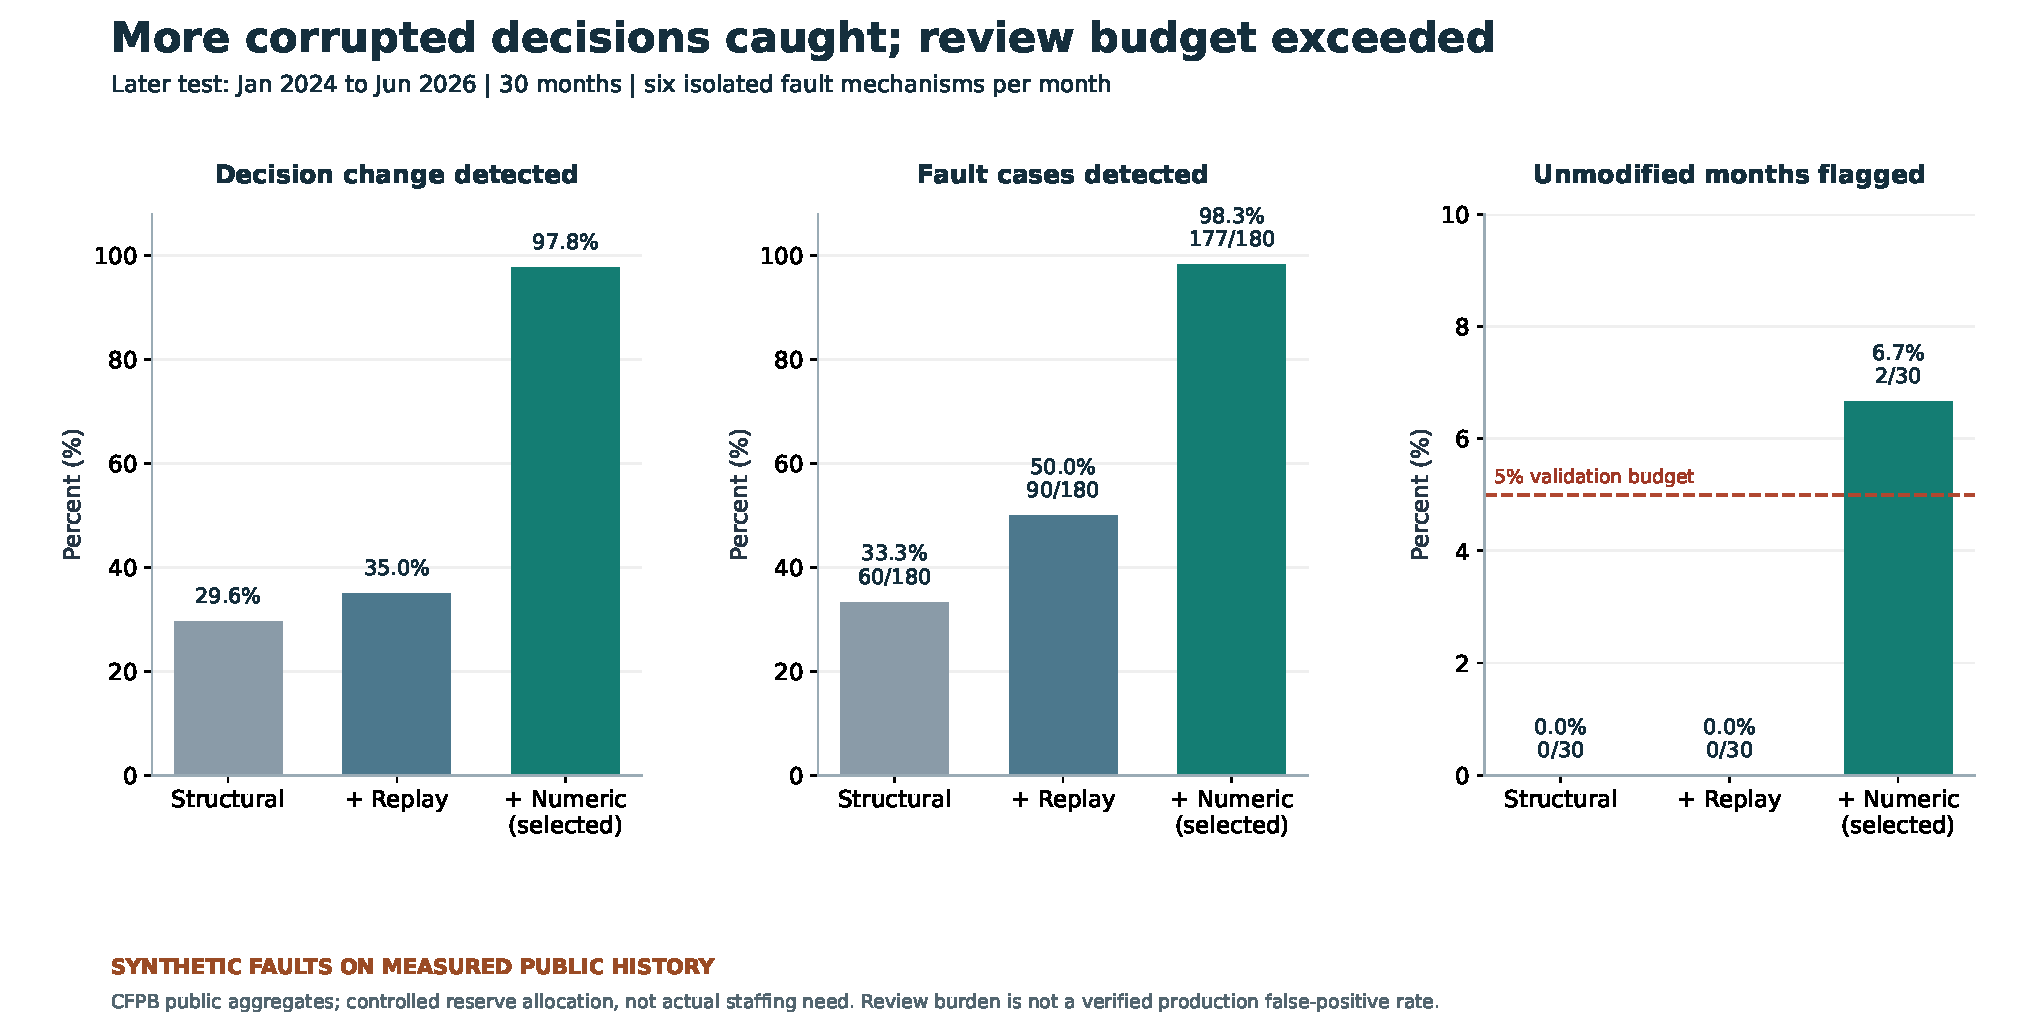
\includegraphics[width=.98\linewidth,height=.85\textheight,keepaspectratio]{images/detection-review-tradeoff.pdf}
\par\small Figure 1. Higher synthetic decision-change detection comes with a later unmodified-history review budget failure. The third panel uses its own clearly labelled scale.
\end{landscape}
\clearpage\begin{landscape}\centering
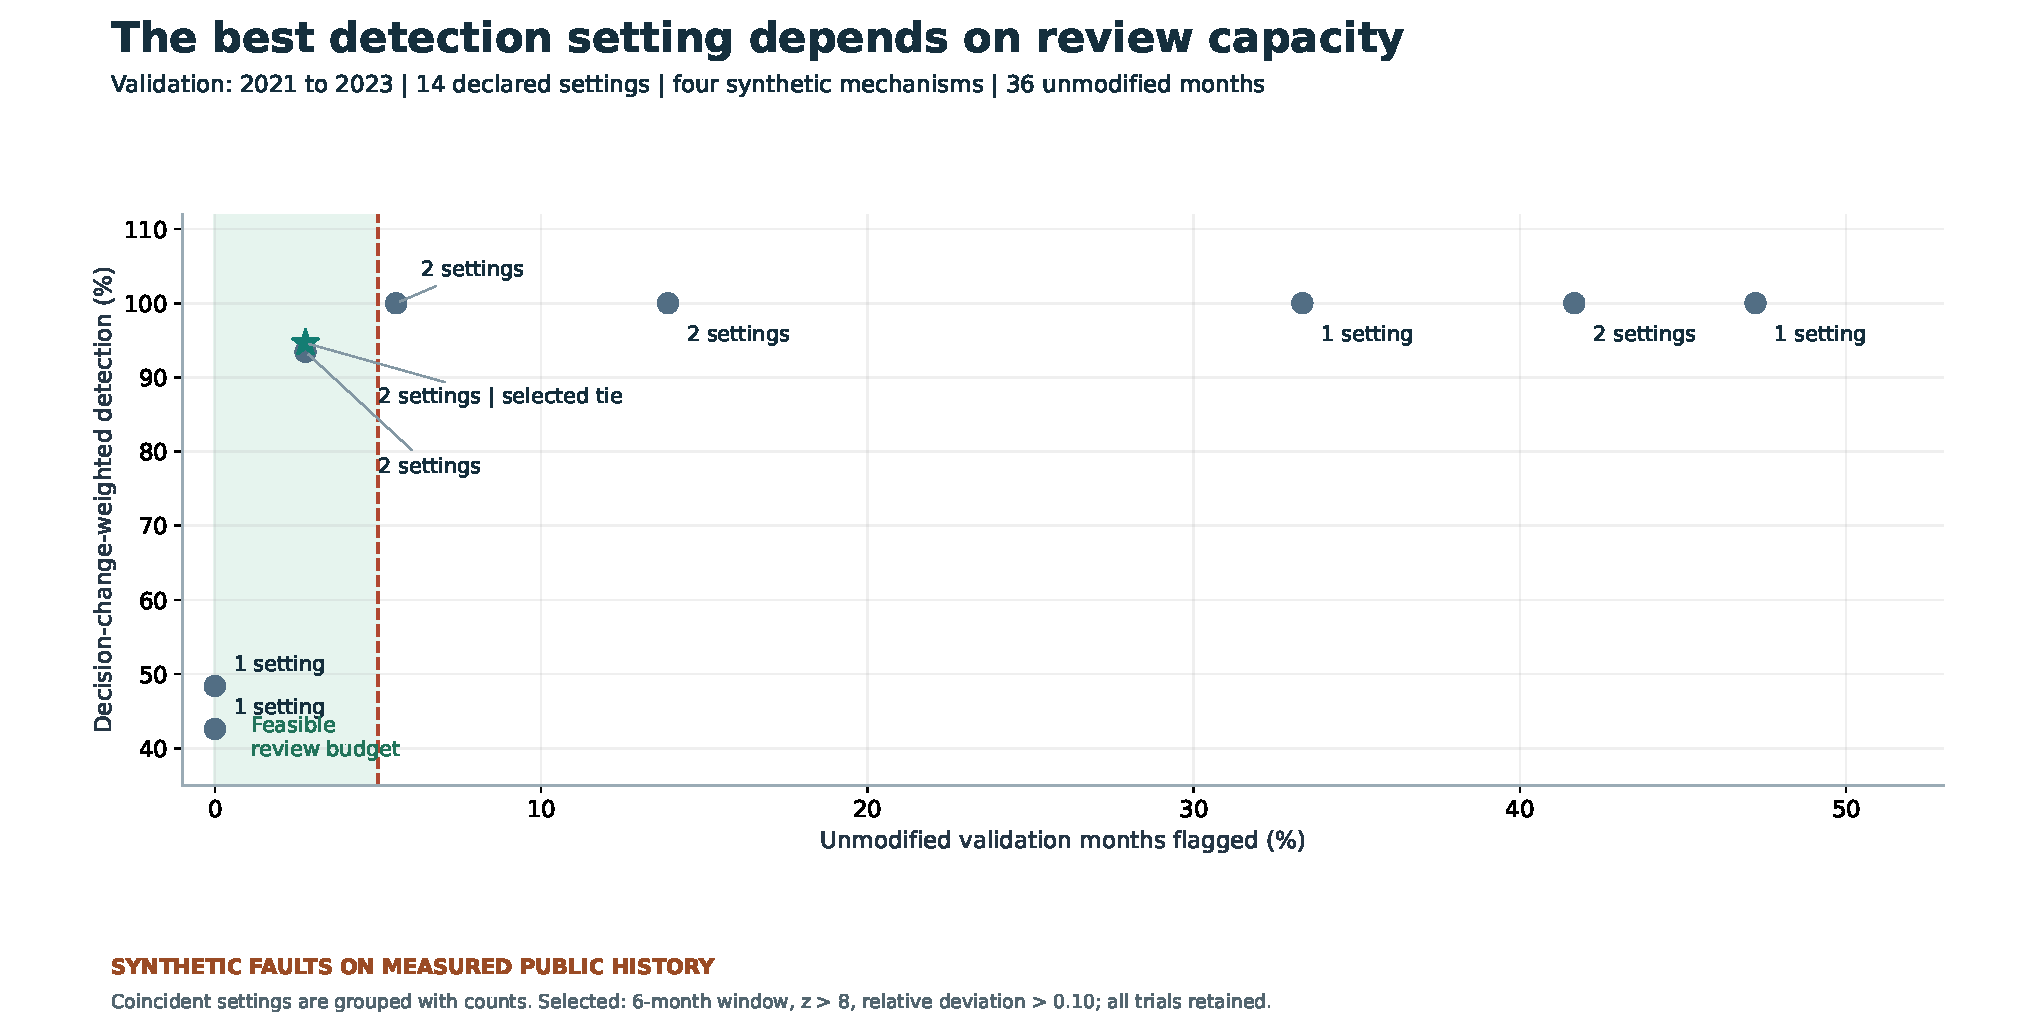
\includegraphics[width=.98\linewidth,height=.85\textheight,keepaspectratio]{images/validation-budget-frontier.pdf}
\par\small Figure 2. All fourteen finite settings are represented; coincident points are grouped with counts. Selection is constrained by review burden, not recall alone.
\end{landscape}
\clearpage\begin{landscape}\centering
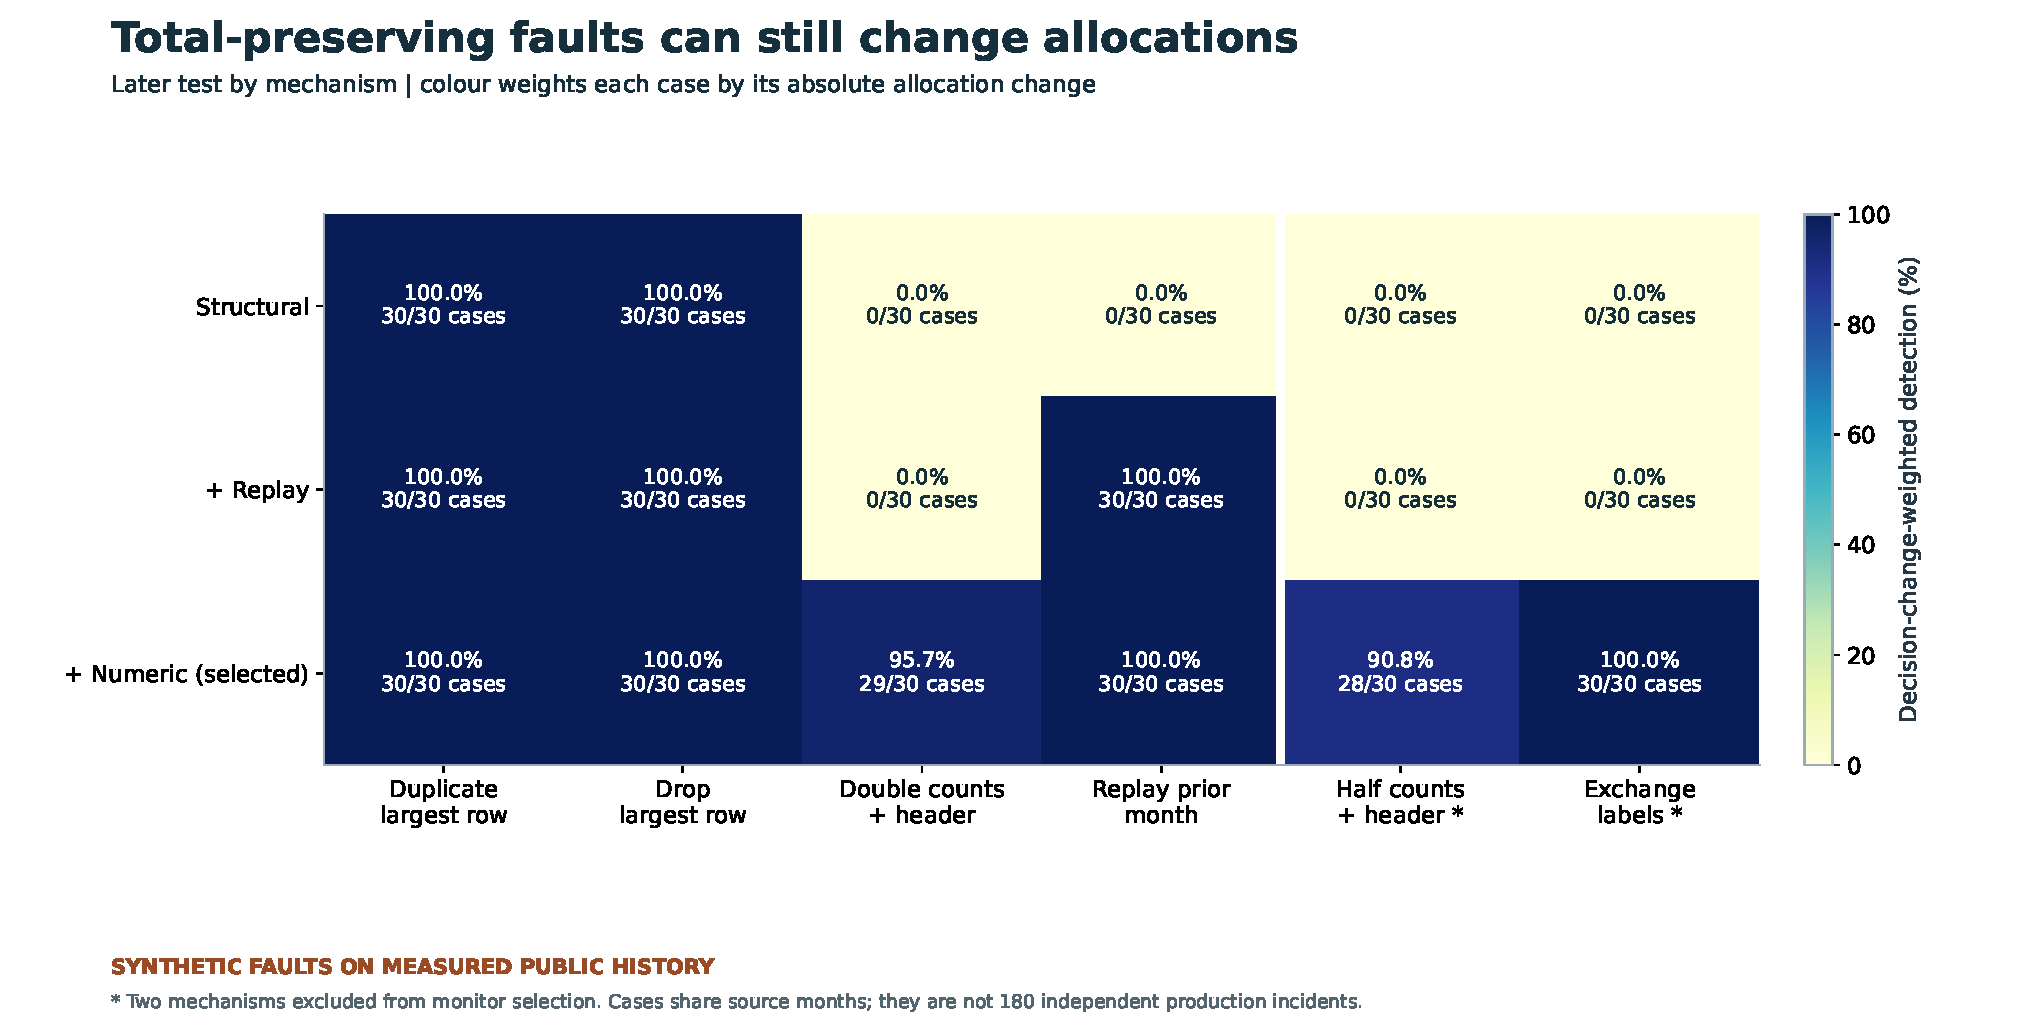
\includegraphics[width=.98\linewidth,height=.85\textheight,keepaspectratio]{images/fault-family-transfer.pdf}
\par\small Figure 3. Total-preserving and header-consistent faults expose a gap in the stated structural checks. Asterisks identify mechanisms excluded from selection.
\end{landscape}
\end{document}
